\section{Chapter 6 - Problem (1)}
	Suppose the coefficient of static friction between the road and the tires on a car is $0.92$. What speed will put the car on the verge of sliding as it rounds a level curve of $83 \ ft$ radius?

	\textbf{R:} \newline

	\begin{figure}[H]
		\begin{center}
			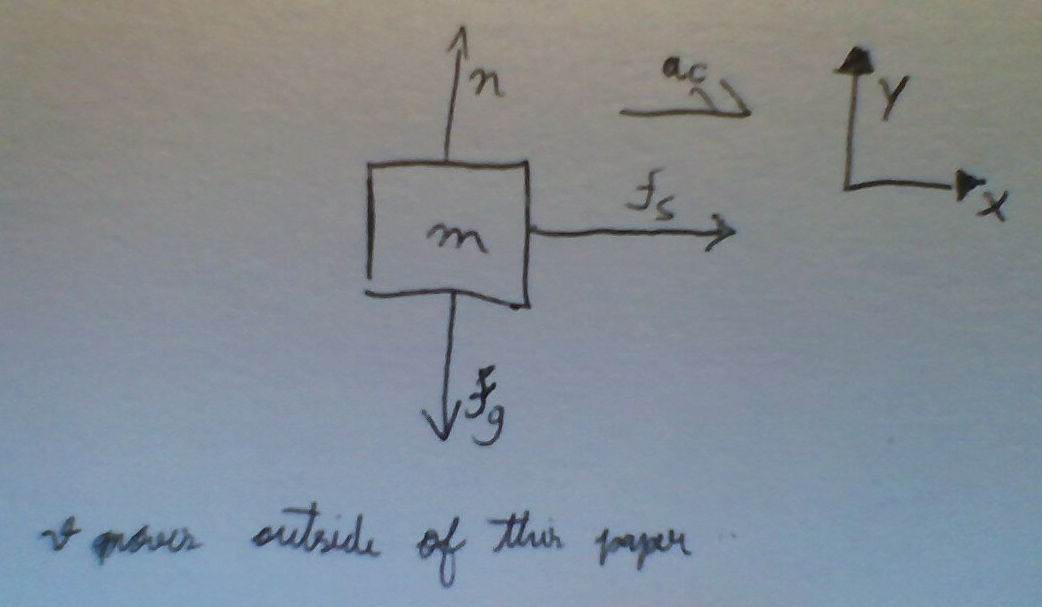
\includegraphics[scale=0.3]{hw6_problem1_fbd}
			\caption{Free-Body Diagram (Problem 1)}
			\label{fig:hw6_problem1_fbd}
		\end{center}
	\end{figure}

	\begin{align}
		f_{s,max} = \ &\mu_{s}n& \notag
	\end{align}

	Newton's $2^{nd}$ Law:

	\begin{align}
		\sum F_{x} = \ &ma_{x}& \notag \\
		f_{s} = \ &ma_{c}& \notag
	\end{align}

	\begin{align}
		\sum F_{y} = \ &ma_{y}& \notag \\
		n - f_{g} = \ &m(0)& \notag \\
		n = \ &f_{g}& \notag
	\end{align}

	\begin{align}
		f_{s} = \ &f_{s,max}& \notag \\
		ma_{c} = \ &\mu_{s}mg& \notag \\
		a_{c} = \ &\mu_{s}g& \notag \\
		= \ &(0.92)\left(32.2 \ ft/s^{2}\right)& \notag \\
		= \ &26.404 \ ft/s^{2}& \notag
	\end{align}

	\begin{align}
		a_{c} = \ &\frac{v^{2}}{r}& \notag \\
		v = \ &\sqrt{a_{c}r}& \notag \\
		= \ &\sqrt{\left(26.404 ft/s^{2}\right)(83 \ ft)}& \notag \\
		= \ &\sqrt{2191.5 \ ft^{2}/s^{2}}& \notag \\
		= \ &46.814 \ ft/s&
	\end{align}
